%!TEX program = xelatex
\documentclass[11pt, a4paper]{article}
  \usepackage[a4paper,top=3cm,bottom=4cm,left=2.5cm,right=2.5cm]{geometry}
  \usepackage{subfig}
  \usepackage{graphicx}
  \graphicspath{{../images/}}
  \usepackage{hyperref}
  \usepackage{amsmath}
  \usepackage{braket}
  \usepackage{enumitem}
  \usepackage{multirow}
  \usepackage{mathtools}
  \usepackage{xepersian}
  \settextfont[Scale=1.2]{B Nazanin}
  \setlatintextfont[Scale=1]{Times New Roman Cyr}
  \title{\textbf{شبیه‌سازی رایانه‌ای در فیزیک}\\تمرین هفتم: مدل آیزینگ}
  \author{سینا معمر ۹۵۱۰۲۳۱۶}
    

\begin{document}

\maketitle
\thispagestyle{empty}


\section{\textbf{شبیه‌سازی مدل آیزینگ}}
کد این بخش را در فایل
\lr{Ising2D}
می‌توان مشاهده نمود.
در این فایل دو کلاس
\lr{Ising2D}
و
\lr{RenderData}
وجود دارد که هر یک در ادامه توضیح داده خواهند شد.
\\
برای ایجاد یک مدل آیزینگ باید ابتدا یک
\lr{object}
از کلاس
\lr{Ising2D}
به طول و پارامتر
$J$
دل‌خواه بسازیم.
در این حالت دمای سیستم بی‌نهایت فرض می‌شود و یک شبکه‌ی تصادفی از اسپین‌های بالا و پایین می‌سازیم.
انرژی و مغناطش کلی شبکه را نیز حساب کرده و در متغیر‌هایی ذخیره می‌کنیم.
بعد از ساختن شبکه نوبت به تحول شبکه برای رسیدن به دمای مورد نظر از طریق روش متروپولیس-مونت کارلو است.
برای این کار باید تابع
\lr{render}
را با دمای و تعداد نمونه‌های معتبر دل‌خواه صدا بزنیم.
باید توجه کرد که دما به طور پیش‌فرض به صورت دمای کاهیده در واحد
$\frac{J}{K_b}$
در نظر گرفته می‌شود.
برای تغییر آن به حالت دمای عادی، باید
\lr{reduced\_unit=False}
را به ورودی تابع بدهیم.
روش کار این تابع به این صورت است که ابتدا به اندازه‌ی
$100$
قدم مونت‌ کارلو جلو می رود و انرژی‌ها را در یک لیست ذخیره می‌کند.
برای انجام قدم‌های مونت کارلو باید تابع
\lr{\_monte\_carlo\_move}
را صدا بزنیم.
این تابع به تعداد خانه‌ها جفت اعداد رندوم در بازه‌ی اندیس شبکه تولید می‌کند و در هر مرحله
با استفاده از تابع
\lr{\_diff\_energy}
تغییر انرژی حاصل از تغییر اسپین این خانه را پیدا می‌کند.
اگر این تغییر انرژی کم‌تر از صفر بود و یا اگر عدد رندوم تولید شده کم‌تر از احتمال متناسب با این تغییر انرژی بود،
اسپین این خانه را معکوس می‌کند و انرژی کل را به اندازه‌ی تغییر انرژی حساب شده،
زیاد می‌کند.
پس از آن
$100$
قدم،
 با استفاده از تابع
\lr{\_relaxation\_time}
زمان واهلش را حساب می کنیم.
اگر این زمان بیش‌تر از
$100$
بود، به اندازه اختلاف آن‌ها دوباره قدم مونت کارلو برداشته و همین روند را تکرار می‌کنیم تا در نهایت زمان واهلش پایدار شود.
سپس سراغ مرحله‌ی نمونه‌گیری می‌رویم.
در این مرحله به تعداد نمونه‌های خواسته شده قدم مونت کارلو برداشته و در هر قدم انرژی، مغناطش و طول هم‌بستگی مکانی را
در لیست متناظر با خودشان ذخیره می‌کنیم.
برای محاسبه‌ی طول هم‌بستگی مکانی از تابع
\lr{spatial\_correlation\_length}
استفاده می‌کنیم.
در انتها پایداری انرژی‌های به دست آمده را با تابع
\lr{\_equilibrium\_time}
حساب می‌کنیم.
اگر جواب به پایداری نرسیده باشد نمونه‌گیری را دوباره تکرار می‌کنیم ولی در صورتی که به پایداری رسیده باشیم،
به اندازه‌ی زمان پایداری به دست آمده دوباره نمونه می‌گیریم و جایگزین نمونه‌های اولیه می‌کنیم.
در آخر یک
\lr{object}
از کلاس
\lr{RenderData}
با اطلاعات شبکه و کمیات حساب شده می‌سازیم و آن را به عنوان خروجی برمی‌گردانیم.
\\
کلاس
\lr{RenderData}
حاوی تمام اطلاعات مشخص‌کننده‌ی شبکه از جمله دما، طول،
$J$،
انرژی‌ها، مغناطش‌ها و طول‌های هم‌بستگی‌ حساب شده است.
این کلاس هم‌چنین شامل توابعی برای حساب کردن
میانگین متغیر‌ها و خطای آن‌ها است.
هم‌چنین می توان با صدا زدن تابع
\lr{save}
اطلاعات را به صورت یک فایل با فرمت
\lr{.npy}
ذخیره کرد و بعدا با استفاده از تابع
\lr{load}
این اطلاعات را خواند و تحلیل نمود.



\section{\textbf{رفتار کمیت‌های ماکروسکوپی شبکه بر حسب دما برای طول‌های مختلف}}
برای این کار باید تابع
\lr{calc\_ising\_macro\_quantities}
را از فایل
\lr{q1.py}
با طول‌ها، بازه‌ی دمایی و تعداد نمونه‌های دل‌خواه صدا بزنیم.
این تابع برای هر طول و هر دما با تعداد نمونه‌های خواسته شده،
تابع
\lr{render}
مدل آیزینگ را صدا می‌زند و داده‌های حاصل را در یک فایل با فرمت
\lr{.npy}
ذخیره می‌کند.
در نهایت این داده‌ها را که شامل کمیات
$\frac{\braket{E}}{N}$،
$\frac{\braket{|M|}}{N}$،
$\frac{C}{N}$،
$\frac{\chi}{N}$
و
$\xi$
هستند را برای همه‌ی طول‌ها در یک نمودار رسم می‌کنیم.
نمودار‌های به دست آمده را در شکل‌های
\ref{fig:ising_e}
تا
\ref{fig:ising_xi}
می‌توان مشاهده نمود.

\paragraph{میانگین انرژی اسپین}
همان طور که در شکل
\ref{fig:ising_e}
دیده می‌شود،
این کمیت در ابعاد مختلف شبکه،
رفتار بسیار مشابهی دارد و منحنی ‌ها تقریبا روی هم قرار گرفته اند.
علاوه بر این طبق انتظاری که از قبل داشتیم،
در دماهای پایین به دلیل هم‌جهت شدن اسپین‌ها،
اسپین‌ها پایین‌ترین انرژی ممکن که
$-2$
است را پیدا می‌کنند.
هم‌چنین در دما‌های بالا به دلیل تصادفی شدن جهت‌گیری‌ها،
میانگین انرژی به صفر میل می‌کند.
علاوه بر این مشاهده می شود که حول دمای بحرانی شیب نمودار افزایش شدید پیدا می‌کند.

\paragraph{میانگین مغناطش اسپین}
همان طور که در شکل
\ref{fig:ising_m}
دیده می‌شود،
این کمیت در دماهای بالاتر از دمای بحرانی مقداری نزدیک به صفر و در دما‌های کم‌تر از آن به
$1$
میل می‌کند.
که این با شهود کلی ما سازگار است.
زیرا در دما‌های بالا به علت تصادفی بودن جهت گیری، مغناطش خالصی نخواهیم داشت ولی
در دما‌های پایین به دلیل هم‌جهت شدن اسپین‌ها،
به حداکثر مقدار ممکن خواهیم رسید.
هم‌چنین مشاهده می‌شود که در نزدیکی دمای بحرانی منحنی رفتار نمایی از خود نشان داده و با شیب زیادی شروع به رشد می‌کند.
در دماهای دور از دمای بحرانی نیز طول‌های مختلف رفتار یکسانی را از خود نشان می‌دهند.

\paragraph{ظرفیت گرمایی اسپین}
همان‌طور که در شکل
\ref{fig:ising_c}
مشاهده می‌شود،
این کمیت در دماهای بالا و پایین نسبت به دمای بحرانی، به صفر میل می‌کند
و در دمای بحرانی شاهد رشد نمایی آن هستیم.
به دلیل محدود بودن ابعاد شبکه ماکزیمم مقدار آن محدود خواهد بود ولی در حالت حدی،
مقدار آن در دمای بحرانی به بی‌نهایت میل خواهد کرد.
در دماهای دور از دمای بحرانی نیز طول‌های مختلف رفتار یکسانی را از خود نشان می‌دهند.

\paragraph{پذیرفتاری مغناطیسی اسپین}
همان‌طور که در شکل
\ref{fig:ising_x}
مشاهده می‌شود،
این کمیت در دماهای بالا و پایین نسبت به دمای بحرانی، به صفر میل می‌کند
و در دمای بحرانی شاهد رشد نمایی آن هستیم.
به دلیل محدود بودن ابعاد شبکه ماکزیمم مقدار آن محدود خواهد بود ولی در حالت حدی،
مقدار آن در دمای بحرانی به بی‌نهایت میل خواهد کرد.
در دماهای دور از دمای بحرانی نیز طول‌های مختلف رفتار یکسانی را از خود نشان می‌دهند.

\paragraph{طول هم‌بستگی مکانی}
همان‌طور که در شکل
\ref{fig:ising_xi}
مشاهده می‌شود،
این کمیت در دماهای بالا و پایین نسبت به دمای بحرانی، به صفر میل می‌کند
و در دمای بحرانی شاهد رشد نمایی آن هستیم.
که این رفتار با شهود ما نیز سازگار است.
زیرا در دما‌های بالا به دلیل تصادفی بودن جهت‌گیری اسپین‌ها،
آن‌ها مستقل از یکدیگر عمل می کنند.
هم‌چنین در دما‌های پایین نیز به علت کم بودن افت و خیز اسپین‌ها،
تغییر جهت یک اسپین روی اسپین‌های کناری تاثیری نخواهد داشت،
به همین دلیل طول هم‌بستگی مکانی در این دو حالت به صفر میل خواهد کرد.
به دلیل محدود بودن ابعاد شبکه ماکزیمم مقدار آن محدود خواهد بود ولی در حالت حدی،
مقدار آن در دمای بحرانی به بی‌نهایت میل خواهد کرد.
در دماهای دور از دمای بحرانی نیز طول‌های مختلف رفتار یکسانی را از خود نشان می‌دهند.

\begin{figure}[h!]
	\centering
  \begin{minipage}[b]{0.48\textwidth}
    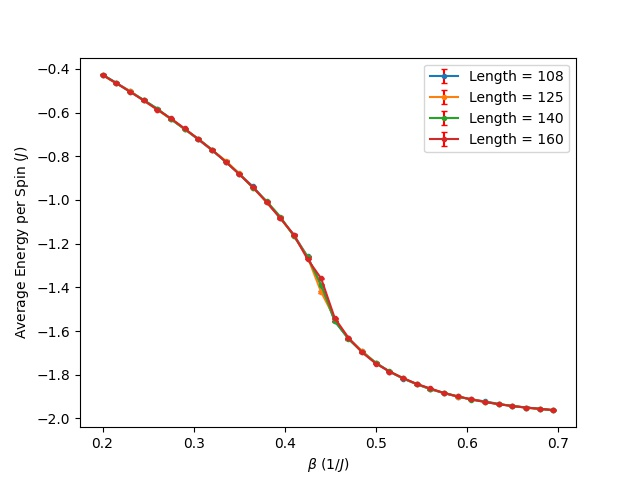
\includegraphics[width=\textwidth]{ising_render_data_e[108, 125, 140, 160]_0.2_0.695_0.015_100.jpg}
    \caption{تغییرات میانگین انرژی اسپین‌ بر حسب $\beta$ در آیزینگ دو بعدی برای طول‌های مختلف شبکه}
    \label{fig:ising_e}
  \end{minipage}
  \hfill
  \begin{minipage}[b]{0.48\textwidth}
    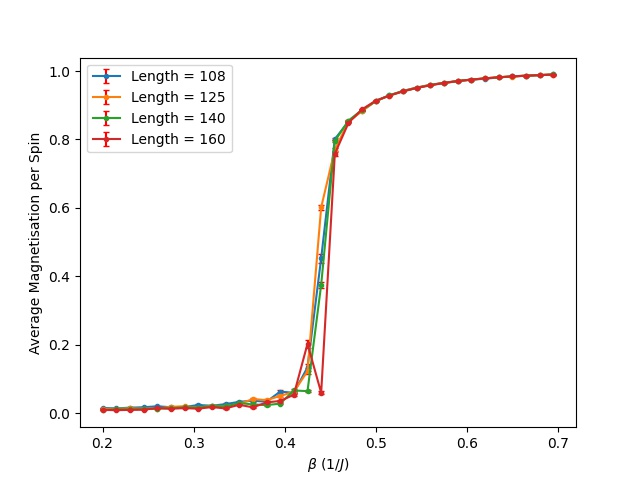
\includegraphics[width=\textwidth]{ising_render_data_m[108, 125, 140, 160]_0.2_0.695_0.015_100.jpg}
    \caption{تغییرات میانگین مغناطش اسپین‌ بر حسب $\beta$ در آیزینگ دو بعدی برای طول‌های مختلف شبکه}
    \label{fig:ising_m}
  \end{minipage}
  \begin{minipage}[b]{0.48\textwidth}
    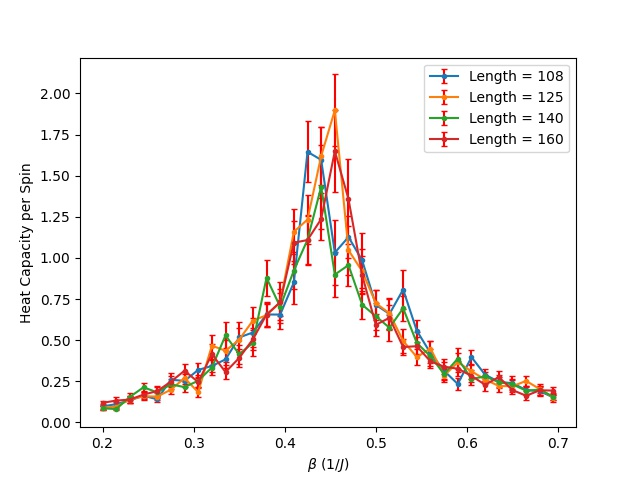
\includegraphics[width=\textwidth]{ising_render_data_c[108, 125, 140, 160]_0.2_0.695_0.015_100.jpg}
    \caption{تغییرات ظرفیت گرمایی اسپین‌ بر حسب $\beta$ در آیزینگ دو بعدی برای طول‌های مختلف شبکه}
    \label{fig:ising_c}
  \end{minipage}
  \hfill
  \begin{minipage}[b]{0.48\textwidth}
    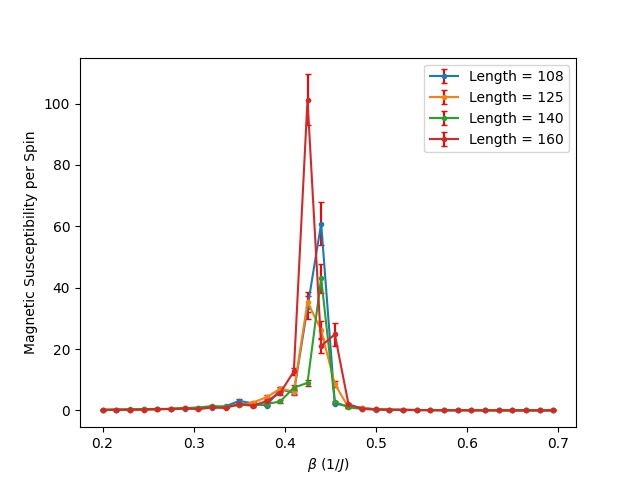
\includegraphics[width=\textwidth]{ising_render_data_x[108, 125, 140, 160]_0.2_0.695_0.015_100.jpg}
    \caption{تغییرات پذیرفتاری مغناطیسی اسپین‌ بر حسب $\beta$ در آیزینگ دو بعدی برای طول‌های مختلف شبکه}
    \label{fig:ising_x}
  \end{minipage}
  \hfill
  \begin{minipage}[b]{0.48\textwidth}
    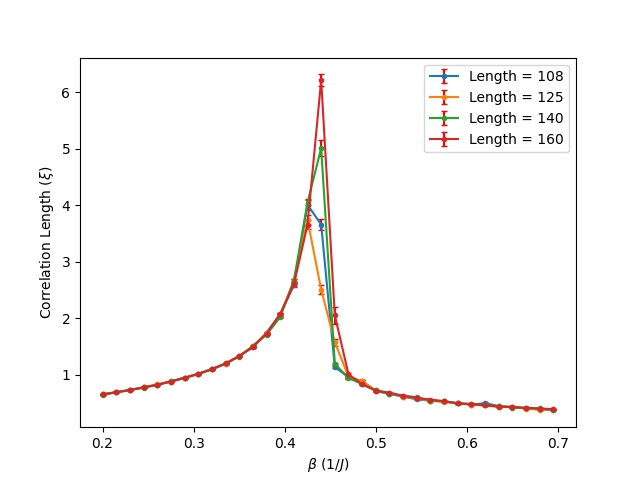
\includegraphics[width=\textwidth]{ising_render_data_xi[108, 125, 140, 160]_0.2_0.695_0.015_100.jpg}
    \caption{تغییرات طول هم‌بستگی مکانی بر حسب $\beta$ در آیزینگ دو بعدی برای طول‌های مختلف شبکه}
    \label{fig:ising_xi}
  \end{minipage}
  \hfill
\end{figure}


\section{\textbf{روش بهینه برای تغییر دمای سیستم در شبیه‌سازی}}
در مدل آیزینگ اگر
$T \gg T_c$
باشد، هیچ هم‌بستگی‌ای بین اسپین‌ها وجود نخواهد داشت و هر اسپین به طور تصادفی در یک جهت قرار خواهد گرفت. و جهت آن نیز به سرعت تغییر خواهد کرد
در نتیجه یک شبکه تصادفی خواهیم داشت.
در صورتی هم که
$T \ll T_c$
باشد، اسپین‌ها دوباره هم‌بستگی چندانی نخواهند داشت ولی برای مینیمم کردن انرژی آزاد،
با همدیگر هم‌جهت خواهند شد و هم‌چنین به دلیل پایین بودن دما،
افت و خیز چندانی نخواهند داشت و جهت‌شان به سختی تغییر خواهد کرد.
همان طور که در قسمت اول ذکر شده،
برای اینکه بتوانیم نمونه‌های معتبری از سیستم داشته باشیم،
باید بگذاریم تا انرژی به حالت تعادل برسد.
از آن‌جایی که حالت تعادل دماهای نزدیک بهم به یکدیگر نزدیک است،
پس در صورتی که برای رفتن به دمای بعدی از شبکه‌ی نهایی به دست آمده در دمای قبلی استفاده کنیم،
با سرعت بیش‌تری به تعادل خواهیم رسید.
حال سوالی که باقی می‌ماند این است که ابتدا باید از دما‌های پایین سیستم را شروع کنیم یا از دماهای بالا؟
اگر قصد بررسی سیستم در دماهای پایین را تنها داشته باشیم،
بهتر است که از یک شبکه‌ی کاملا هم‌جهت شروع کنیم.
ولی در صورتی که قصد بررسی دماهای بالا و یا بررسی یک رنج دمایی از دماهای زیاد تا کم را داشته باشیم،
بهترین انتخاب یک شبکه‌ی تصادفی است.
زیرا یک شبکه تصادفی معادل با دماهای زیاد است و در نتیجه اسپین‌ها به راحتی تغییر جهت خواهند داد و به شبکه نهایی خواهیم رسید.
از آن‌جایی که در این سوال قصد بررسی رفتار کمیت‌های سیستم در یک بازه‌ی نسبتا گسترده‌ی دمایی را داریم،
از یک شبکه‌ی تصادفی که معادل با دماهای بالا است شروع کرده و برای هر دمای جدید،
از شبکه‌ی به دست آمده در دمای قبلی استفاده می‌کنیم.



\section{\textbf{محاسبه‌ی نماهای بحرانی و ضریب $C_0$}}
از تئوری می‌دانیم که میزان مقدار پیک ظرفیت‌ گرمایی، پذیرفتاری مغناطیسی و طول هم‌بستگی در ابعاد محدود،
با افزایش طول شبکه باید به طور یک‌نواخت افزایش پیدا کند.
ولی همان‌طور که در شکل‌های
\ref{fig:ising_c}
تا
\ref{fig:ising_xi}
مشاهده می شود، در نتایج به دست آمده‌ی ما،
این رفتار دیده نمی‌شود و مقدار ماکزیمم به صورت نامنظم زیاد و و کم می‌شود.
علت این موضوع این است که با افزایش طول شبکه،
این نمودارها به حالت شبکه بی‌نهایت نزدیک‌تر می‌شوند و منحنی در حول نقطه‌ی بحرانی بسیار تیز می‌گردد.
در اثر این تیز شدن منحنی، با انحراف بسیار کوچکی از نقطه‌ی بحرانی،
مقدار کمیت به شدت افت می‌کند.
به همین دلیل برای پیدا کردن مقدار ماکزیمم حقیقی نیاز به تعیین مقدار نقطه بحرانی با دقت بالا می‌باشد.
برای تعیین این مقدار بحرانی در طول‌های مختلف تلاش زیادی انجام شد و حتی با دقت
$0.001$
کمیت
$\beta$
تغییر داده شد ولی نتایج به دست آمده باز هم در طول‌های بالاتر رفتار نامنظم داشتند و نمای بحرانی به دست آمده از آن‌ها،
با مقدار حقیقی به شدت تفاوت داشت.
نتایج به دست آمده به صورت فایل‌هایی
\lr{.npy}
در پوشه‌ی
\lr{data}
موجود می ‌باشند و با استفاده از تابع
\lr{calc\_ising\_macro\_quantities}
و پاس دادن آرگومان
\lr{file\_name="file name"}
می‌توان آن‌ها را مشاهده نمود.
\\
با توجه به این توضیحات داده شده،
تصمیم بر آن شد که شبیه‌سازی را برای طول‌های کوچک‌تر انجام دهیم تا بتوان با دقت بالا مقدار ماکزیمم را در این کمیات به دست آورد.
برای طول های کوچک‌تر از
$8$
منحنی حالت تیز‌شدگی خود را از دست می داد و امکان تعیین ماکزیمم با دقت لازم نبود.
به همین دلیل شبیه‌سازی را برای طول‌های
$8$،
$16$،
$32$
و
$64$
انجام دادیم.
نتایج به دست آمده برای نقطه‌ی بحرانی و مقدار ماکزیمم کمیت‌ها در این‌ طول‌ها را در جدول
\ref{tab:critical_T_max}
می‌توان مشاهده نمود.
از روی این مقادیر می توان نمودار‌های
\ref{fig:l_T}
تا
\ref{fig:m_l}
را رسم نمود و از روی شیب خط فیت شده به آن‌ها،
نماهای بحرانی را محاسبه نمود.
نماهای به دست آمده به صورت زیر هستند:

\begin{equation}
  \nu = 0.72
  \label{eqn:nu}
\end{equation}

\begin{equation}
  \frac{\gamma}{\nu} = 1.75
  \xRightarrow{\eqref{eqn:nu}}
  \gamma = 1.26
\end{equation}

\begin{equation}
  \frac{C_0}{\nu} = -0.61
  \xRightarrow{\eqref{eqn:nu}}
  C_0 = -0.44
\end{equation}

\begin{equation}
  \frac{\beta}{\nu} = 0.20
  \xRightarrow{\eqref{eqn:nu}}
  \beta = 0.142
\end{equation}

\begin{table}[h!]
  \centering
  \begin{tabular}{|c|c|c|c|c|c|c|c|c|}
    \hline
    \multicolumn{2}{|c|}{$64$} & \multicolumn{2}{c|}{$32$} & \multicolumn{2}{c|}{$16$} & \multicolumn{2}{c|}{$8$} & \multirow{2}{*}{$l$} \\  \cline{1-8}
    \lr{max}     &      $T_c$     &       \lr{max}    &     $T_c$      &       \lr{max}    &      $T_c$     &     \lr{max}      &      $T_c$     &  \\ \hline
        $2.60$      &     $2.30$      &      $2.15$     &     $2.29$      &     $1.77$      &      $2.28$     &     $1.32$      &     $2.35$      & $C / N$ \\ \hline
        $74.88$      &     $2.31$      &      $22.67$     &     $2.32$      &     $6.95$      &      $2.40$     &     $1.94$      &     $2.49$      & $\chi / N$ \\ \hline
        $5.28$      &     $2.30$      &      $2.39$     &     $2.35$      &     $1.47$      &      $2.45$     &     $0.88$      &     $2.84$      & $\xi$ \\ \hline
  \end{tabular}
  \caption{نقاط بحرانی و ماکزیمم کمیات برای طول‌های مختلف شبکه‌ی آیزینگ دو بعدی}
  \label{tab:critical_T_max}
\end{table}

\begin{figure}[h!]
	\centering
  \begin{minipage}[b]{0.48\textwidth}
    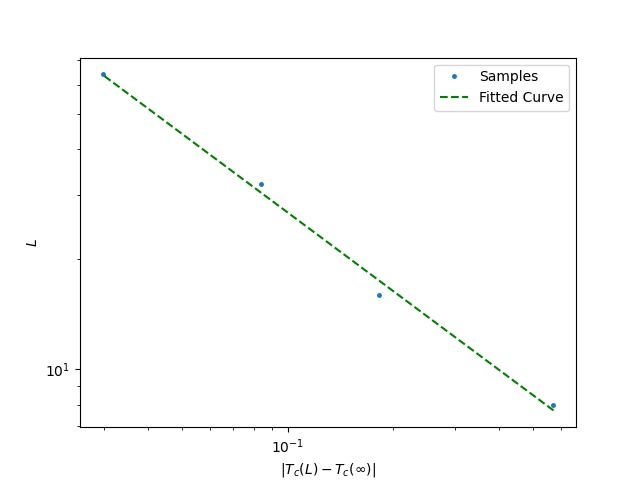
\includegraphics[width=\textwidth]{nu.jpg}
    \caption{تغییرات $L$ بر حسب $|T_c(L) - T_c(\infty)|$ در شبکه آیزینگ دو بعدی}
    \label{fig:l_T}
  \end{minipage}
  \hfill
  \begin{minipage}[b]{0.48\textwidth}
    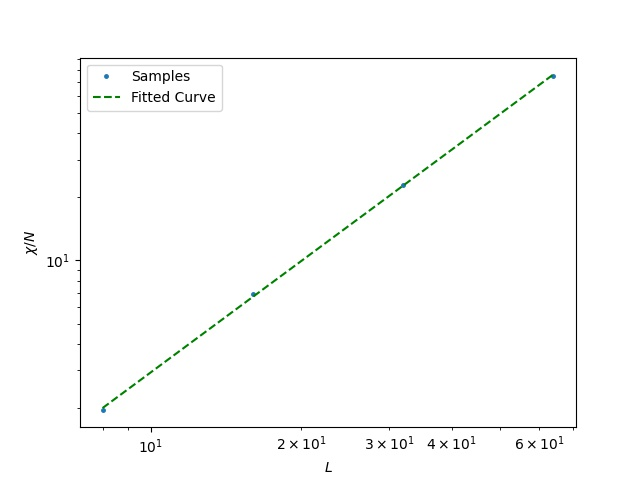
\includegraphics[width=\textwidth]{gamma.jpg}
    \caption{تغییرات $\chi / N$ در نقطه‌ی بحرانی بر حسب طول شبکه آیزینگ دو بعدی}
    \label{fig:xi_l}
  \end{minipage}
  \begin{minipage}[b]{0.48\textwidth}
    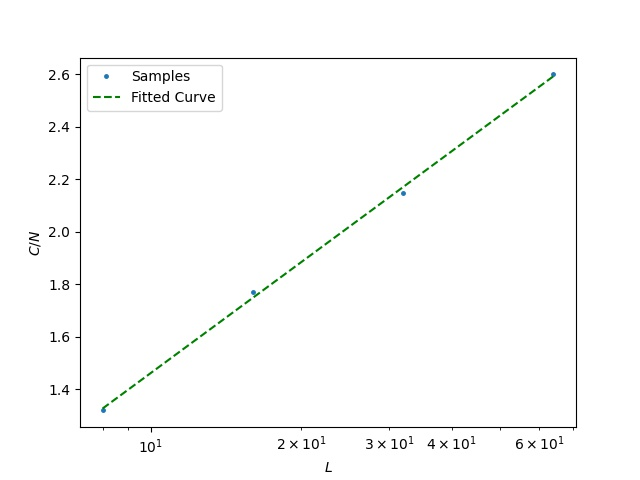
\includegraphics[width=\textwidth]{c_0.jpg}
    \caption{تغییرات $C / N$ در نقطه‌ی بحرانی بر حسب طول شبکه آیزینگ دو بعدی}
    \label{fig:c_l}
  \end{minipage}
  \hfill
  \begin{minipage}[b]{0.48\textwidth}
    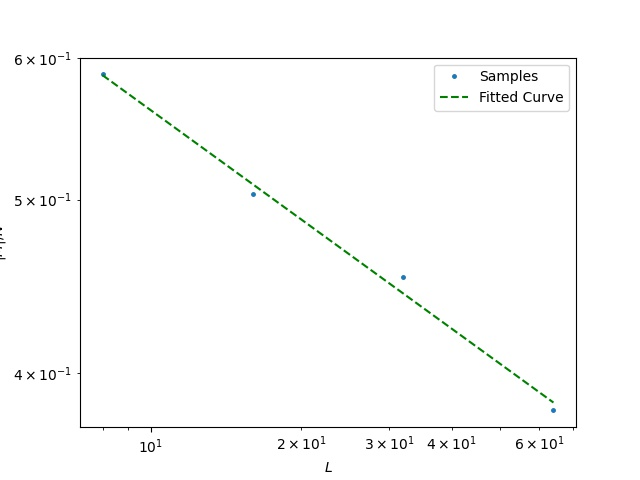
\includegraphics[width=\textwidth]{beta.jpg}
    \caption{تغییرات $|M| / N$ در نقطه‌ی بحرانی بر حسب طول شبکه آیزینگ دو بعدی}
    \label{fig:m_l}
  \end{minipage}
  \hfill
\end{figure}



\section{\textbf{تغییرات شبکه بر حسب دما (امتیازی)}}
برای مشاهده تغییرات شبکه بر حسب دما،
یک مدل آیزینگ به طول
$108$
می‌سازیم و آن را از
$\beta = 0.2$
تا
$\beta = 0.7$
با قدم‌های
$0.015$
و با
$100$
داده معتبر نمونه‌گیری،
شبیه‌سازی می‌کنیم و با استفاده از تابع
\lr{show}
شکل گرافیکی آن را به دست می‌آوریم.
در نهایت شکل‌های به دست آمده را تبدیل به گیف می‌کنیم تا روند تغییرات دمایی به طور واضح دیده شود.
فایل مورد نظر را در پوشه
\lr{images}
تحت عنوان
\lr{ising\_108\_grids\_Ts.gif}
می‌توان مشاهده نمود.



\end{document}
